\documentclass{article}

\usepackage[utf8]{inputenc}
\usepackage[T1]{fontenc}
\usepackage{lipsum}
\usepackage{graphicx}
\usepackage{amsmath}
\usepackage[margin=1in]{geometry}
\usepackage{titlesec}
\usepackage{graphicx}
\usepackage{floatflt,epsfig}
\usepackage[utf8]{inputenc}
\usepackage[T1]{fontenc}
\usepackage{lipsum}
\usepackage{graphicx}
\usepackage{amsmath}
\usepackage[margin=1in]{geometry} 
\usepackage{titlesec}
\usepackage{listings}
\usepackage{xcolor}

\lstdefinelanguage{XML}
{
  morestring=[b]",
  morestring=[s]{>}{<},
  morecomment=[s]{<?}{?>},
  morecomment=[s][\color{green!50!black}]{<!--}{-->},
  stringstyle=\color{blue},
  identifierstyle=\color{red},
  keywordstyle=\color{orange},
  commentstyle=\color{green!50!black},
  basicstyle=\small\ttfamily,
  frame=single, 
  breaklines=true,
  breakatwhitespace=true,
  tabsize=2,
  showstringspaces=false,
  captionpos=b,
}

\lstdefinelanguage{Java}{
  keywords={abstract,assert,boolean,break,byte,case,catch,char,class,const,continue,default,do,double,else,enum,extends,false,final,finally,float,for,goto,if,implements,import,instanceof,int,interface,long,native,new,null,package,private,protected,public,return,short,static,strictfp,super,switch,synchronized,this,throw,throws,transient,true,try,void,volatile,while},
  morekeywords={[2]System,out},
  morecomment=[l]{//},
  morecomment=[s]{/*}{*/},
  morestring=[b]",
  basicstyle=\small\ttfamily,
  keywordstyle=\color{blue}\bfseries,
  keywordstyle={[2]\color{orange}\bfseries},
  commentstyle=\color{green!70!black},
  stringstyle=\color{red},
  showstringspaces=false,
  tabsize=2,
  breaklines=true,
  breakatwhitespace=true,
  frame=single, 
  captionpos=b
}


\titleformat{\section}
{\LARGE\bfseries}{\thesection}{1em}{}

\titleformat{\subsection}
{\Large\bfseries}{\thesection}{1em}{}

\begin{document}

\pagestyle{empty}

\section*{Activity}
\large

Le \textbf{activities} rappresentano una parte fondamentale all'interno di \textit{Android Studio}, data la loro importanza in questo contesto. Spesso le \textit{activities} sono raffigurate come il primo contatto tra il sistema software realizzato e l'utente, da cui sono sviluppati metodi o funzioni in grado di poter acquisire dati provenienti da agenti esterni. Articolando l'introduzione, le stesse sono note anche secondo la denominazione \textbf{screen state}, ossia un fotogramma in grado di intrappolare tutto ciò che riesca a contraddistinguere il preciso momento in cui si trovi lo screen del dispositivo. \vspace*{14pt}\\
Concludendo \textit{Android} stabilisce la sua operatività mediante uno \textbf{stack} di activity, infatti le medesime applicazioni si basano sul susseguirsi di insiemi di \textit{attività}.\vspace*{14pt}\\
Le \textbf{activity} devono essere dichiarate all'interno del \textbf{Manifest}, contenitore di informazioni estremamente importanti a livello di sistema operativo; pertanto, occorre che siano descritte all'interno del Manifest prima che siano runnate, anche se solitamente, a seconda della versione di \textit{Android Studio}, tutto ciò è definito automaticamente.
\begin{lstlisting}[language=XML, title=Dichiarazione di un'activity all'interno del Manifest]
<application ...>
  <activity android:name=".MainActivity" android:exported="true">
    <intent-filter>
      <action android:name="android.intent.action.MAIN" />
      <category android:name="android.intent.category.LAUNCHER" />
    </intent-filter>
  </activity>
</application>
\end{lstlisting}
Il \textit{Manifest} indica ciò che il sistema operativo possa visionare in riferimento all'applicazione che si trovi in stato \textit{running}; proprio per questa principale motivazione, la sezione \textit{XML} riportata precedentemente, definisce quali e come utilizzare le attività formulate al suo interno.

\subsection*{Activity Lifecycle} 
Le \textbf{activity} nel corso del loro \textit{lifecycle}, attraversano una sequenzialità di \textit{stati}, adottati per differenti contesti, soprattutto data la volontà di distinguere quale delle differenti operazioni debba essere svolta. Infatti l'operazione, o meglio definito \textit{elemento computazionale}, raffigura l'unico item in grado di mantenere in vita l'applicazione circoscritta, per cui una gestione dei propri stati indica una sezione imprescindibile.\vspace*{14pt}\\
Come da immagine sottostante, si evidenziano un totale di cinque stati, di cui \textit{destroyed} non è da considerarsi tale. In relazione, si prosegue attraverso una semplice descrizione di ognuno di essi, la lettura scaturisce sin dal momento in cui l'attività non risulti essere in memoria.
\begin{enumerate}
  \renewcommand{\labelenumi}{-}
  \item \textbf{Created}, in questo istante l'\textit{activity} non risulta ancora visibile, si tratta di una fase precedente al \textit{running}, ma non alla compilazione
  \item \textbf{Started}, stato successivo in cui l'attività è visibile ma non ancora funzionante, o meglio non è interagibile, non riesce ancora a comunicare ed acquisire eventi generati da fattori esterni
  \item \textbf{Resumed}, l'\textit{activity} è in "primo piano", del tutto funzionante e pertanto interagibile
  \item \textbf{Paused}, si verifica l'\textit{overlaid} di altre attività, un esempio concreto potrebbe essere un'\textit{interrupt} generata da uno specifico evento caratterizzato da una maggiore priorità, il quale necessita di assimilare un livello e numero superiore di risorse, da cui scaturisce il fenomeno che provocherà lo stato descritto
  \item \textbf{Stopped}, in comune allo stato precedente, l'attività non può eseguire alcuna sezione di codice oppure ricevere dati, in aggiunta non risulta più visibile poichè portata in "secondo piano"
\end{enumerate}   
\begin{center}
  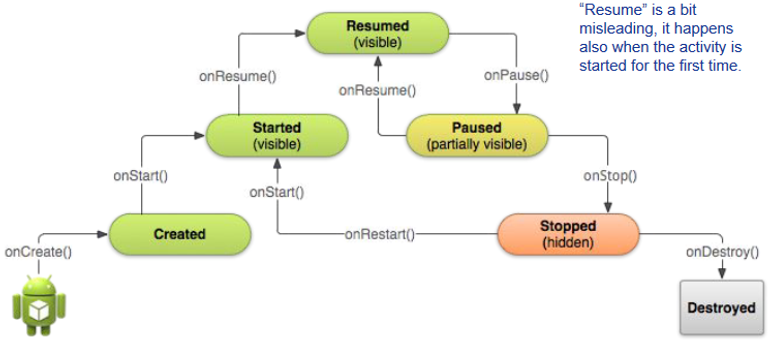
\includegraphics[width=0.7\textwidth]{foto1.png}
\end{center}
Detto ciò, l'insieme di caratteristiche riportate è dovuto all'avvenire di certi eventi, per lo più provocati da specifici metodi; secondo questa breve deduzione, si intuisce la presenza di molteplici funzioni che possano provocare i differenti passaggi di stato. Anche in questa circostanza suddivisi in:
\begin{enumerate}
  \itemsep0em 
  \renewcommand{\labelenumi}{-}
  \item \textbf{onCreate()}, funzione richiamata nel momento in cui l'\textit{activity} viene creata; solitamente contiene le sezioni di codice necessarie per imbastire l'intera logica dell'attività, pertanto sono eseguite solamente ad una occorenza. Inoltre è definito come il principale responsabile per la designazione della \textit{user interface}
  \item \textbf{onStart()}, metodo successivo a \textit{onCreate()}, interpellato poco prima che la finestra principale sia visibile all'utente e pertanto interagibile
  \item \textbf{onResume()}, come avviene per lo stato descritto prima, la funzione circoscritta definisce tutti i componenti affinchè l'\textit{activity} possa essere \textit{runnata}; terminata la propria computazione l'attività potrà essere eseguita
  \item \textbf{onPause()}, interviene qualora l'attività dovesse essere interrotta, a livello esemplificativo si evince attraverso un'interrupt a livello di priorità di processi; tipicamente non consegue con alcuna memorizzazione, data la sua estrema velocità di passaggio, tuttavia permette allo scheduler della CPU di rimuovere tutti i processi relativi all'attività affinchè non consumino risorse computazionali. Rispetto a quanto detto, l'attività risulta ancora visibile ma solo parzialmente, ossia tendenzialmente è applicata una velatura opaca per simboleggiarne l'inattività
  \item \textbf{onRestart()}, adottato solo quando l'\textit{activity} sia momentaneamente sospesa oppure stoppata
  \item \textbf{onStop()}, l'attività non è più visibile e di conseguenza interagibile, spesso fenomeno causato da due fattori specifici; la prima causa potrebbe essere dedotta da uno "spostamento" in \textit{background} di un'activity in favore di una corrisposta, oppure l'attività è in procinto di essere distrutta
  \item \textbf{onDestroy()}, funzione attuata qualora il sistema necessiti dello spazio in memoria oppure, con maggiore semplicità, qualche elemento ha chiamato il metodo circoscritto sulla precisa attività
\end{enumerate}   
Tuttavia è bene definire che i molteplici passaggi di stato sono controllati in minima parte dallo sviluppatore, da cui si evince l'importanza di saper almeno riconoscere il comportamento di un'attività durante il proprio \textit{lifecycle}.
\subsection*{Logs with LogCat}
Questa breve sezione si concentra sulla tematica denominata \textbf{logcat window}, usufruito come un vero e proprio strumento che possa aiutare qualsiasi sviluppatore durante l'implementazione di certe funzionalità, attuato principalmente durante attività di \textit{debugging}; ad esempio potrebbero essere aggiunti alcuni messaggi all'applicazione sviluppata mediante l'estensione della \textit{classe log}.\vspace*{14pt}\\
La \textit{classe log} predispone un'elevato numero di metodi che possano definire l'importanza del messaggio di log visualizzato.
\begin{lstlisting}[language=JAVA, title=Dichiarazione dei log]
Log.v ("LABEL", "message")    // VERBOSE
Log.d ("LABEL", "message")    // DEBUG
Log.i ("LABEL", "message")    // INFORMATION
Log.w ("LABEL", "message")    // WARNING
Log.e ("LABEL", "message")    // ERROR
Log.wtf ("LABEL", "message")  // SHOULD NEVER HAPPEN IN LIFE
\end{lstlisting}

\subsection*{Recreating Activities}
Qualora si navigasse tra le differenti \textit{activities} che compongono l'applicazione in questione, il sistema, tendenzialmente, adotta un approccio distruttivo dell'attività per poi, successivamente, crearne una nuova istanza. Un andamento simile provoca un sovraccarico a livello operativo, necessita uno strumento in grado di ricreare l'attività senza che essa sia sottoposta all'iter precedente. In tal senso è adoperato un \textit{bundle}, denominato \textbf{instance state}, responsabilizzato della memorizzazione delle \textit{activities}, da cui l'applicativo avrà la possibilità di riesumarne l'oggetto ogni qual volta ne avesse la possibilità.\vspace*{14pt}\\
Il salvataggio dei dati circoscritti avviene tramite l'\textit{override} di due metodi principali, definiti come segue:
\begin{enumerate}
  \itemsep0em 
  \renewcommand{\labelenumi}{ }
  \item \textbf{onSaveInstanceState()}, generalmente metodo richiamato poco prima che l'\textit{activity} sia posta in \textit{stopped}
  \begin{lstlisting}[language=JAVA, title=Salvataggio dei dati poco prima dello stato stopped]
static final String STATE_SCORE = "playerScore";
@Override
public void onSaveInstanceState (Bundle savedInstanceState) {
  super.onSaveInstanceState (savedInstanceState);
  savedInstanceState.putInt(
    STATE_SCORE, mCurrentScore
  );
}
  \end{lstlisting}
  \item \textbf{onRestoreInstanceState()}, funzione richiamata poco dopo che l'attività sia posta in \textit{started}
  \begin{lstlisting}[language=JAVA, title=Salvataggio dei dati poco dopo dello stato started]
@Override
public void onRestoreInstanceState (Bundle savedInstanceState) {
  // Call the superclass to restore the views
  super.onRestoreInstanceState (savedInstanceState);
  mCurrentScore = savedInstanceState.getInt(STATE_SCORE);
}
  \end{lstlisting}
\end{enumerate}
In alternativa, i due metodi elencati, possono essere adeguati anche durante la fase di creazione dell'\textit{activity}. 

\subsection*{Task e BackStack}
Le attività, durante il lifecycle di un'applicazione, concorrono tra di loro, posizionandosi visivamente al di sopra. In questo caso, l'attività precedente, ossia da poco sostituita da una propria corrisposta, viene salvata all'interno del \textbf{BackStack}\vspace*{7pt}\\
Il \textit{BackStack} opera come una pila, pertanto secondo il funzionamento \textit{FIFO}; navigando tra le differenti componenti dell'applicazione l'utente estrae l'attività corrente all'interno dello stack, distruggendola, e ricrea l'\textit{activity} posizionata al di sopra della pila.\vspace*{7pt}\\
Tuttavia, potrebbe sorgere un problema legato all'esecuzione della stessa attività in due differenti fasi della medesima storyline, provocando, in tal contesto, la creazione di due differenti istanze; un esempio è dettato dall'utilizzo della mail-box, in cui si evidenzia un'\textit{activity} usufruita per la visualizzazione del contenuto e una seconda adottata per la scrittura di un messaggio, per cui stessa attività ma due istanze differenti. Per evitare un caso simile, è possibile forzare il sistema affinchè non crei due istanze della stessa classe, mediante l'impiego di \textit{flag}.\vspace*{14pt}\\
Come già accenato, navigare tra le differenti componenti obbliga lo sviluppatore a gestire le molteplici \textit{activities}, spostando la \textbf{task} corrente in secondo piano.\\
Una \textit{task} rappresenta un'unità coesiva, contenitrice di un \textit{BackStack}, posizionata in primo piano oppure in secondo piano, a seconda che l'attività sia in stato \textit{running} oppure \textit{stopped}.\vspace*{7pt}\\
Generalmente la modellazione di task avviene per precise funzioni, da cui per ogni attività è possibile svilupparne il comportamento, modificando un'elevata molteplicità di parametri; contrariamente, eseguire un'applicazione dalla schermata home del dispositivo definisce sempre la stesso approccio.

\subsection*{Contexts}
Un'attività è fortemente connessa ad un contesto, descritto come un punto di interazione tra app e sistema operativo, da cui qualunque entità ha la possibilità di richiamare le sue funzioni.\\
\end{document}